\chapter{Лабораторная работа №6. Реализация корреляционного устройства на ПЛИС}

\section{Сжатие сигналов с применением быстрой свёрки}

Сжатие сигналов — это метод обработки сигналов, используемый в радиолокационных, гидроакустических, сейсмических и других «зондирующих» системах. В данном контексте под «зондирующей» системой понимается система, в которой сигнал передается, отражается от удаленного объекта и принимается для измерения параметров объекта. Сжатие импульсов позволяет максимизировать отношение сигнал/шум и полученить высокое разрешение воспринимаемого объекта (например, для достижения чувствительного обнаружения цели или хорошего качества изображения). 

Современных решением для сжатия сложных сигналов является цифровая быстрая свёртка в спектральной области на основе БПФ. Алгоритм быстрой свёртки имеет следующий вид:

\begin{equation}	
	y(k) = IFFT[FFT\{x(k)\} \cdot \compconj{FFT\{S(k)\}}],
\end{equation}

где y(k) - отсчёты сжатаго сигнала; x(n) - отсчёты эхо-сигналов, то есть отражённый от целей;
S(k) - отсчёты, описывающие зондирующий сигнал(опорная функция). Блок-схема алгоритма приведена на рисунке ~\ref{fft_conv}.

\begin{figure}[h]
	\centering
	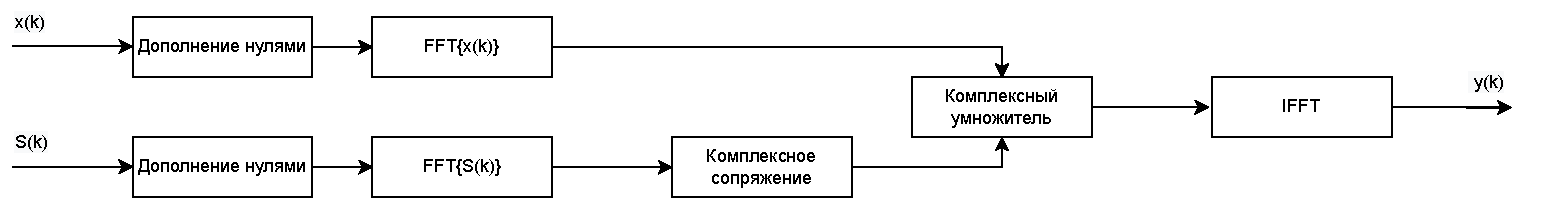
\includegraphics[width=0.9\textwidth]{fft_conv.pdf}
	\caption{Блок-схема алгоритма быстрой свёртки}
	\label{fft_conv}
\end{figure}

Данный алгоритм сжатия (свертки) сложных сигналов и сама система сжатия имеет большие преимущества перед согласованными фильтрами, так как легко адаптируется к виду сигнала, его ширине спектра, обладает большим динамическим диапазоном и легко реализуется при использовании современных цифровых компонентов, особенно программируемых логических интегральных схем (ПЛИС).

В радиолокационных системах широкое применение находит сигнал с линейной-частотной модуляцией, поэтому рассмотрим процесс сжатия на примере ЛЧМ-сигнала.

\section{Сжатие ЛЧМ-сигнала}

Сигнал с линейной-частотной модуляцией определяется по следующей формуле:
\begin{equation}	
	s(t) = rect(\frac{t}{T}) \cdot \cos(2 \cdot \pi \cdot f_0 \cdot t + j \cdot \pi \cdot K \cdot t^{2}),
\end{equation}

где t - время в секундах, K-скорость изменения частоты во времени, T - длительность импульса, rect() - прямоугольное окно, \(f_0\) - несущая частота.

После прохождения через квадратурный демодулятор получаем следующий комплексный сигнал:

\begin{equation}	
	g(t) = rect(\frac{t}{T}) \cdot \exp(j \cdot \pi \cdot K \cdot t^{2})
\end{equation}

Действительная часть называется квадратурной
составляющей ЛЧМ-сигнал, и обозначается как \(Q(t)\), а мнимая 
синфазной составляющей ЛЧМ-сигнала, и обозначается как \(I(t)\):

\begin{equation}	
	Q(t) = rect(\frac{t}{T}) \cdot \cos(\pi \cdot K \cdot t^{2}),
\end{equation}

\begin{equation}	
	I(t) = rect(\frac{t}{T}) \cdot \sin(\pi \cdot K \cdot t^{2}).
\end{equation}

Важнейшими параметрами ЛЧМ-сигнала являются:

\begin{enumerate}
	\item Девиация частоты: 
\begin{equation}
	BW = |K| \cdot T, 
\end{equation}
измеряется в Гц.
	\item База: 
\begin{equation}
	B = |K| \cdot T^2, 
\end{equation}
безразмерная величина.
\end{enumerate}

Рассмотрим конкретный пример демодулированного ЛЧМ-сигнала. Пусть он имеет следующие параметры: частота дискретизации \(F_{D}\) = 1000 МГц, девиация частоты \(BW\) = 400 МГц, длительность сигнала \(T\) = 4 мкс. На рисунке ~\ref{fig:chirp} представлена квадратурная и синфазная составляющая ЛЧМ-сигнала с приведёнными выше параметрами. 

Проведём моделирование отражённого от цели сигнала. При распространении сигнала возникает временная задержка, накладывается шум, а также происходит затухание сигнала. Введём некоторую временную задержку, а также наложим на сигнал белый шум. При наложении белого шума будем руководствоватся заданным отношение сигнал/шум на уровне 0 Дб. На рисунке ~\ref{fig:chirp_shift} представлена сдвинутая по времени копия ЛЧМ-сигнала, а на рисунке ~\ref{fig:chirp_shift_noise} представлен этот же сдвинутый сигнал, но уже при наличии шума.  

Проведём сжатие данного сигнала на основе формулы представленной в предыдущем параграфе. Для этого:

\begin{enumerate}
	\item Находим быстрое преобразование Фурье эталонного сигнала(рис. ~\ref{fig:chirp}), выполняем комплексное сопряжение полученного массива.
	\item Находим быстрое преобразование Фурье отражённого от цели (в терминах радиолокации) сигнала (рис. ~\ref{fig:chirp_shift_noise}).
	\item Производим комплексное умножение полученных массивов.
	\item Находим обратное быстрое преобразование Фурье.
\end{enumerate}

На рисунке ~\ref{fig:correl} представлены квадратурная и синфазная составляющая сжатого сигнала. При этом прослеживается чёткий пик, не смотря на наличие шума. Эта помехоустойчивость достигается за счет того, что фильтр согласуется только с сигналом, а не с шумом — он не коррелирует с шумом. Согласованный фильтр «собирает» большую часть компонентов сигнала в один пик, но оставляет шумовые компоненты случайным образом распределенными в выходном массиве. Известно, что при наличии гауссовского аддитивного шума оптимальным приемником с точки зрения максимизации отношения сигнал/шум на пике сжатого импульса является приемник с согласованным фильтром.

\begin{figure}[h]
    \centering
    \noindent
    \begin{tikzpicture}
        \begin{axis}
            [
            RCS Plot,
            title={},
            height=0.35\textwidth,
            xlabel={Время, мкс},
            ylabel={Амплитуда, отсчётов},
            legend pos = south east
            ]
            \addplot table {Synopsis/data/third-party/lfm_im.dat};
            \addlegendentry{Q(t)};
            \addplot table {Synopsis/data/third-party/lfm_re.dat};
            \addlegendentry{I(t)};
        \end{axis}
    \end{tikzpicture}
    \caption{Квадратурная и синфазная составляющая ЛЧМ сигнала}
    \label{fig:chirp}
\end{figure}

\begin{figure}[h]
    \centering
    \noindent
    \begin{tikzpicture}
        \begin{axis}
            [
            RCS Plot,
            title={},
            height=0.35\textwidth,
            xlabel={Время, мкс},
            ylabel={Амплитуда, отсчётов},
            legend pos = south east
            ]
            \addplot table {Synopsis/data/third-party/lfm_shift_im.dat};
            \addlegendentry{Q(t)};
            \addplot table {Synopsis/data/third-party/lfm_shift_re.dat};
            \addlegendentry{I(t)};
        \end{axis}
    \end{tikzpicture}
    \caption{Квадратурная и синфазная составляющая задерженного ЛЧМ сигнала}
    \label{fig:chirp_shift}
\end{figure}

\begin{figure}[h]
    \centering
    \noindent
    \begin{tikzpicture}
        \begin{axis}
            [
            RCS Plot,
            title={},
            height=0.35\textwidth,
            xlabel={Время, мкс},
            ylabel={Амплитуда, отсчётов},
            legend pos = south east
            ]
            \addplot table {Synopsis/data/third-party/lfm_shift_noise_im.dat};
            \addlegendentry{Q(t)};
            \addplot table {Synopsis/data/third-party/lfm_shift_noise_re.dat};
            \addlegendentry{I(t)};
        \end{axis}
    \end{tikzpicture}
    \caption{Квадратурная и синфазная составляющая задержненного ЛЧМ сигнала при наличии шума}
    \label{fig:chirp_shift_noise}
\end{figure}

\begin{figure}[h]
    \centering
    \noindent
    \begin{tikzpicture}
        \begin{axis}
            [
            RCS Plot,
            title={},
            height=0.35\textwidth,
            xlabel={Время, мкс},
            ylabel={Амплитуда, отсчётов},
            legend pos = south east
            ]
            \addplot table {Synopsis/data/third-party/correl_re.dat};
            \addlegendentry{I(t)};
			\addplot table {Synopsis/data/third-party/correl_im.dat};
            \addlegendentry{I(t)};
        \end{axis}
    \end{tikzpicture}
    \caption{Квадратурная и синфазная составляющая сигнала на выходе фильтра сжатия}
    \label{fig:correl}
\end{figure}

\section{Выполнение быстрого преобразование Фурье на ПЛИС}

Для реализации БПФ на ПЛИС используем стандартное ядро, которое предоставляет Xilinx.

\subsection{Возможности ядра}

Данное ядро может выполнять быстрое преобразование Фурье входных массивов данных с размером от 8 до 65536 отсчётов, при этом размер преобразуемый данных может быть постоянным, а может изменяться в реальном времени при использовании соответствующего режима. Обработка может выполняться как в режиме с плавающей точкой(на самом деле нет, только приближении к этому режиму, о этом ниже), так и режиме с фиксированной точкой. Также поддерживается обработка одновременно до 16 каналов данных. При вычислении БПФ с фиксированной точкой поддерживается маштабирование, в режиме с плавающей точкой оно игнорируется. 

Ядро БПФ предлагает четыре варианта архитектуры, обеспечивающие компромисс между ресурсами, которые будет занимать ядро на ПЛИС и пропускной способностью ядра (как правило, каждая архитектура предлагает двухкратную разницу в ресурсах по сравнению со следующей архитектурой): 
\begin{enumerate}
	\item Конвейерный потоковый ввод-вывод(Pipelined Streaming I/O) — обеспечивает непрерывную обработку данных. 
	\item Radix-4 — загружает и обрабатывает данные отдельно, используя итеративный подход. Оно меньше по размеру, чем конвейерное решение, но имеет большее время преобразования. 
	\item Radix-2 — использует тот же итеративный подход, что и Radix-4, но бабочка меньше. Это означает, что он меньше по размеру, чем решение Radix-4, но время преобразования больше. 
	\item Radix-2 Lite Burst I/O — основанный на архитектуре Radix-2, этот вариант использует подход с временным мультиплексированием к бабочке для еще меньшего ядра за счет более длительного времени преобразования.
\end{enumerate} 

Каждая архитектура имеет возможность естественного или бит-реверсного порядка выходных данных, в то время как входнные данные вводятся всегда в естественном порядке. Алгоритм БПФ переупорядочивает входные данные во время обработки таким образом, что данные, вводимые в естественном порядке, выводятся в бит-реверсном порядке. Заметим что вывод в естестенном порядке требует дополнительного времени преобразования и дополнительных ресурсов на ПЛИС. В архитектурах Radix-2 Burst I/O, Radix-2 Lite Burst I/O и Pipelined Streaming I/O бит-реверсный порядок битов легко вычислить, взяв индекс точки данных, записанный в двоичном виде, и реверсивное преобразование. порядок цифр. Следовательно, 0000, 0001, 0010, 0011, 0100,... (0, 1, 2, 3, 4,...) становятся 0000, 1000, 0100, 1100, 0010,... (0, 8, 4, 12, 2,...). В случае архитектуры Radix-4 реверсирование применяется к цифрам и поэтому называется реверсированием цифр. Цифра в Radix-4 состоит из двух битов. Следовательно, 0000, 0001, 0010, 0011, 0100,... (0, 1, 2, 3, 4,...) становятся 0000, 0100, 1000, 1100, 0001,... (0, 4, 8). , 12, 1,...), поскольку пары цифр меняются местами. 

\begin{figure}[h]
	\centering
	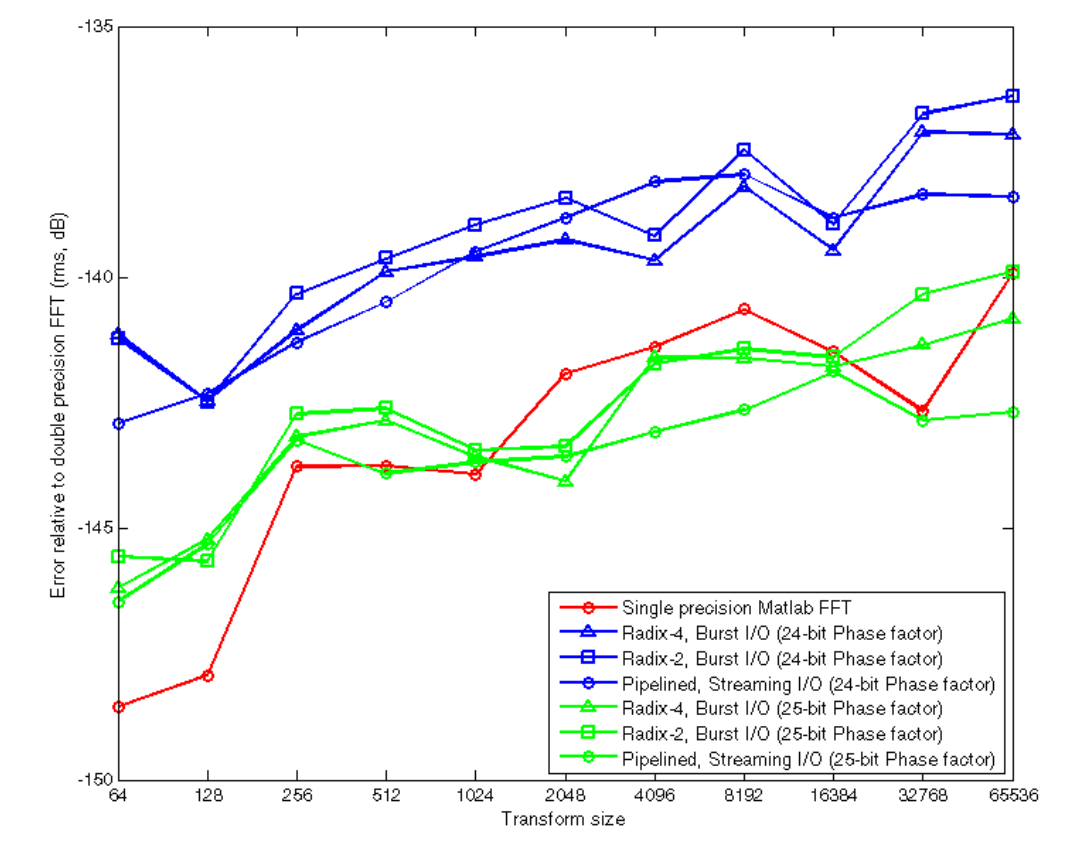
\includegraphics[width=0.6\textwidth]{image/fft_xilinx_fp.png}
	\caption{Сравнение двух уровней шумовых характеристик}
	\label{fft_xilinx_fp}
\end{figure}

Ядро БПФ может принимать данные в формате одинарной точности IEEE-754 с 32-битными словами, состоящими из 1-бита знака, 8-битной экспоненты и 23-битной дроби. Реализация полной плавающей точки на ПЛИС является дорогостоящей с точки зрения требуемых ресурсов. Режим с плавающей точкой использует БПФ с фиксированной запятой более высокой точности для достижения шумовых характеристик, аналогичных полному БПФ с плавающей точкой, со значительно меньшими ресурсами. Рисунок~\ref{fft_xilinx_fp} иллюстрирует два возможных уровня шумовых характеристик при выборе 24 или 25 битов для ширины фазового коэффициента. При увеличении ширины фазового коэффициента до 25 бит может потребоваться больше ресурсов в зависимости от целевого устройства. Таким образом для достижения наибольшей точности вычислений в режиме с плавающей точкой требуется выбирать ширину фазового коэффициента равной 25 бит при наличии ресурсов необходимых для этого.

\subsection{Порты ввода/вывода}

Рассмотреним порты ввода/вывода. 

Для настройки ядра используется интерфейс AXI4-Stream \verb|S_AXIS_CONFIG|. 
Он состоит из следующих линий ввода/вывода: \verb|s_axis_config_tdata| - шина данных,
\verb|s_axis_config_tvalid|, \verb|s_axis_config_tready| - линии механизма "рукопожатий" в интерфейсе AXI4.

\begin{figure}[h]
	\centering
	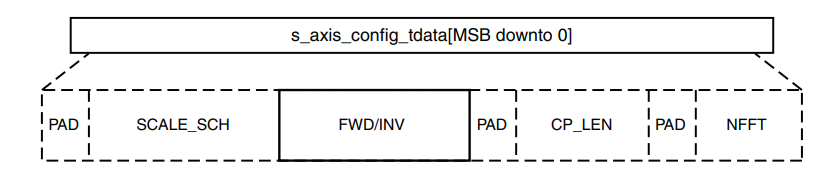
\includegraphics[width=0.5\textwidth]{image/FFT_AXIS_CONFIG.png}
	\caption{Временная диаграмма работы интерфейса AXI4-Stream}
	\label{fft_detailed_implem}
\end{figure}

\begin{figure}[h]
	\centering
	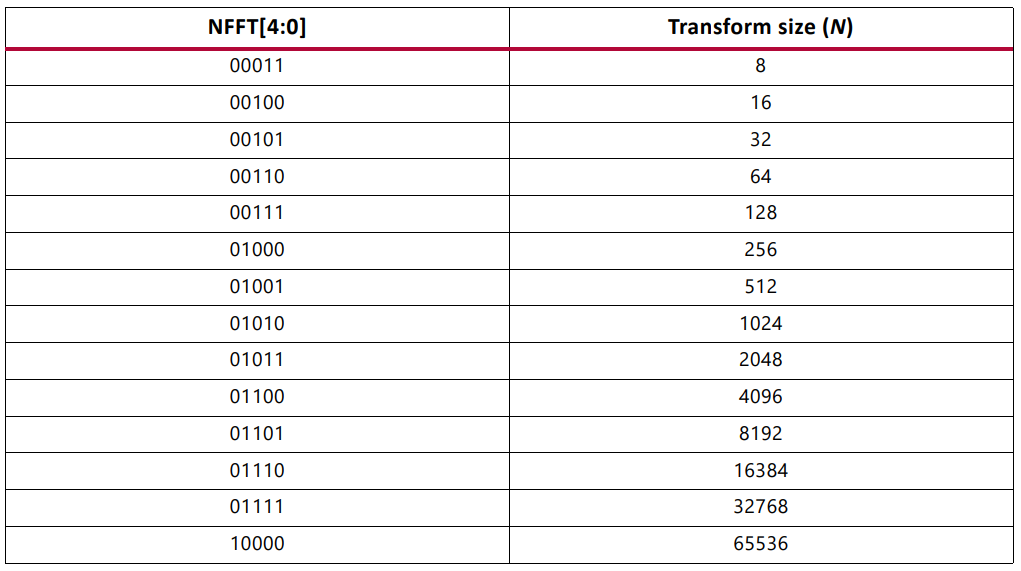
\includegraphics[width=0.5\textwidth]{image/FFT_LENGTH.PNG}
	\caption{Временная диаграмма работы интерфейса AXI4-Stream}
	\label{fft_detailed_implem}
\end{figure}

\begin{enumerate}
	\item Размер точки преобразования: NFFT может быть размером максимального преобразования или любым меньшим размером точки. Например, 1024-точечное БПФ может вычислять размеры точек 1024, 512, 256 и т. д. Значение NFFT равно log2 (размер в пунктах). Это поле присутствует только для размера точки преобразования, настраиваемого во время выполнения.
	Размер точки преобразования можно установить в поле NFFT в канале конфигурации, если выбран параметр длины преобразования, настраиваемая во время выполнения. Допустимые настройки и соответствующие размеры преобразования представлены в таблице 3-18. Если введенное значение NFFT слишком велико, ядро устанавливает максимально доступный размер точки (выбранный в среде IDE). Если значение слишком мало, ядро устанавливает наименьший доступный размер точки: 64 для архитектуры Burst I/O Radix-4 и 8 для других архитектур.
	\item Длина циклического префикса: количество выборок с конца преобразования, которые изначально выводятся как циклический префикс, прежде чем будет выведено все преобразование. \verb|CP_LEN| может быть любым числом от нуля до единицы меньше размера пункта. Это поле присутствует только при вставке циклического префикса.
	\item Указывает, выполняется ли прямое преобразование БПФ или обратное преобразование БПФ. Когда \verb|FWD_INV| = 1, вычисляется прямое преобразование. Если \verb|FWD_INV| = 0, вычисляется обратное преобразование. Поле содержит 1 бит на канал данных БПФ, бит 0 (LSB) представляет канал 0, бит 1 представляет канал 1 и т. д.
	\item График масштабирования: для архитектур пакетного ввода-вывода график масштабирования задается двумя битами для каждого этапа, при этом масштабирование для первого этапа задается двумя младшими битами. Масштабирование может быть указано как 3, 2, 1 или 0, что представляет количество битов для сдвига. Примерный график масштабирования для N = 1024, пакетный ввод-вывод Radix-4: [1 0 2 3 2] (в порядке от последнего к первому этапу). Для N = 128, Radix-2 Burst I/O или Radix-2 Lite Burst I/O, один из возможных графиков масштабирования — [1 1 1 1 0 1 2] (в порядке от последнего к первому этапу). Для архитектуры Pipelined Streaming I/O график масштабирования определяется двумя битами для каждой пары этапов Radix-2, начиная с двух младших разрядов. Например, график масштабирования для N = 256 может быть [2 2 2 3]. Когда N не является степенью числа 4, максимальный прирост битов для последней стадии равен одному биту. Например, [0 2 2 2 2] или [1 2 2 2 2] являются допустимыми расписаниями масштабирования для N = 512, но [2 2 2 2 2] недействительны. Для этой длины преобразования два старших бита \verb|SCALE_SCH| могут быть только 00 или 01. Это поле доступно только с масштабированной арифметикой (не немасштабированной, блочной с плавающей запятой или одинарной точности с плавающей запятой).
\end{enumerate} 

Тип преобразования (прямое или обратное) и график масштабирования можно задавать покадрово, не прерывая обработку кадра. Как тип преобразования, так и график масштабирования могут быть установлены независимо для каждого канала БПФ в многоканальном ядре. Каждому каналу данных FFT назначено поле \verb|FWD_INV| и поле \verb|SCALE_SCH| в канале конфигурации. 
Установка поля \verb|FWD_INV| на 0 создает обратное БПФ, а установка поля \verb|FWD_INV| на 1 создает прямое преобразование. Расписание масштабирования не требуется (\verb|SCALE_SCH| игнорируется), когда ядро FFT настроено на обработку данных с плавающей запятой. Нормализация и масштабирование выполняются внутри для данных с плавающей запятой.

Поля конфигурации упаковываются в вектор \verb|s_axis_config_tdata| в следующем порядке (начиная с младшего разряда):

1. (необязательно) NFFT плюс заполнение 2. (необязательно) \verb|CP_LEN| плюс заполнение 3. FWD/INV 4. (необязательно) \verb|SCALE_SCH|

\begin{enumerate}
	\item \verb|event_frame_started| Этот сигнал события устанавливается в течение одного тактового цикла, когда ядро начинает обрабатывать новый кадр. Этот сигнал предназначен для подсчета кадров и синхронизации конфигурации ядра с конкретным кадром, если это необходимо.
	\item \verb|event_tlast_missing|
	Этот сигнал события устанавливается в течение одного тактового цикла, когда \verb|s_axis_data_tlast| имеет значение Low для последней входящей выборки данных кадра. Это показывает несоответствие конфигурации между ядром и вышестоящим источником данных в отношении размера кадра и указывает, что вышестоящий источник данных настроен на больший размер точки, чем ядро. Это вычисляется только тогда, когда ядро начинает обработку кадра, поэтому событие может отставать от отсутствующего \verb|s_axis_data_tlast| на большое количество тактов.
	\item \verb|event_tlast_unexpected|
	Этот сигнал события утверждается в течение одного тактового цикла, когда ядро видит \verb|s_axis_data_tlast| High для любой входящей выборки данных, которая не является последней в кадре. Это показывает несоответствие конфигурации между ядром и восходящим источником данных в отношении размера кадра и указывает, что восходящий источник данных настроен на меньший размер точки, чем ядро. Это вычисляется только тогда, когда ядро начинает обработку кадра, поэтому событие может отставать от неожиданного High на \verb|s_axis_data_tlast| на большое количество тактовых циклов. Если на \verb|s_axis_data_tlast| для кадра есть несколько неожиданных максимумов, то это утверждается для каждого из них.
	\item \verb|event_fft_overflow|
	Этот сигнал о событии устанавливается в каждом тактовом цикле, когда наблюдается переполнение в выборках данных, передаваемых на \verb|m_axis_data_tdata|. Переполнение БПФ возможно только при использовании масштабированной арифметики или ввода-вывода с плавающей запятой одинарной точности. Во всех других конфигурациях штифт удаляется из сердечника.
	\item \verb|event_data_in_channel_halt|
	Это событие подтверждается в каждом цикле, когда ядру требуются данные из канала ввода данных, а данные недоступны. • В режиме реального времени ядро продолжает обработку кадра, даже если он безвозвратно поврежден. • В режиме не в реальном времени основная обработка останавливается и продолжается только тогда, когда данные записываются в канал ввода данных. Рамка не повреждена. В обоих режимах событие остается подтвержденным до тех пор, пока данные не будут доступны в канале ввода данных.
	\item \verb|event_data_out_channel_halt|
	Это событие подтверждается в каждом цикле, когда ядру необходимо записать данные в канал вывода данных, но это невозможно, потому что буферы в канале заполнены. Когда это происходит, основная обработка останавливается, и вся деятельность останавливается до тех пор, пока в буферах канала не освободится место. Рамка не повреждена. Пин-код события доступен только в режиме не в реальном времени.
	\item \verb|event_status_channel_halt|
	Это событие подтверждается в каждом цикле, когда ядру необходимо записать данные в канал состояния, но это невозможно, потому что буферы в канале заполнены. Когда это происходит, основная обработка останавливается, и вся деятельность останавливается до тех пор, пока в буферах канала не появится свободное место. Кадр не поврежден. Пин-код события доступен только в режиме не в реальном времени.
\end{enumerate}

\subsection{Создание и настройка ядра}

\begin{figure}[h]
	\centering
	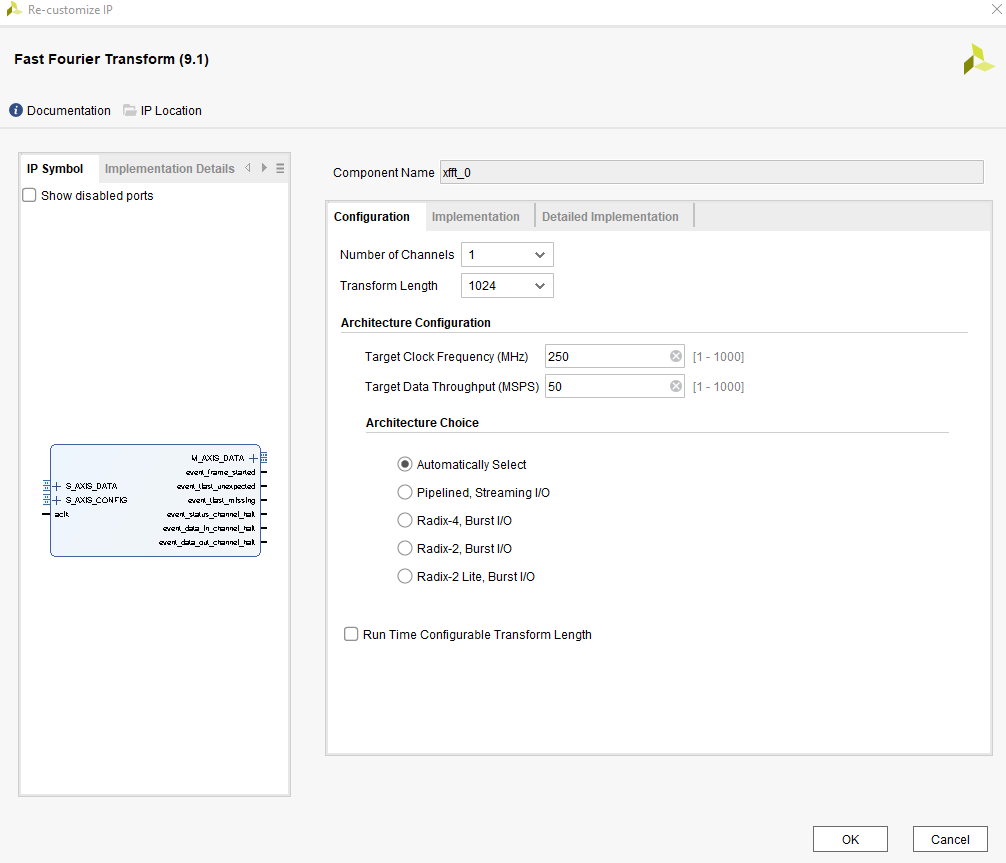
\includegraphics[width=0.5\textwidth]{image/fft_config.png}
	\caption{Временная диаграмма работы интерфейса AXI4-Stream}
	\label{fft_config}
\end{figure}
	
\begin{figure}[h]
	\centering
	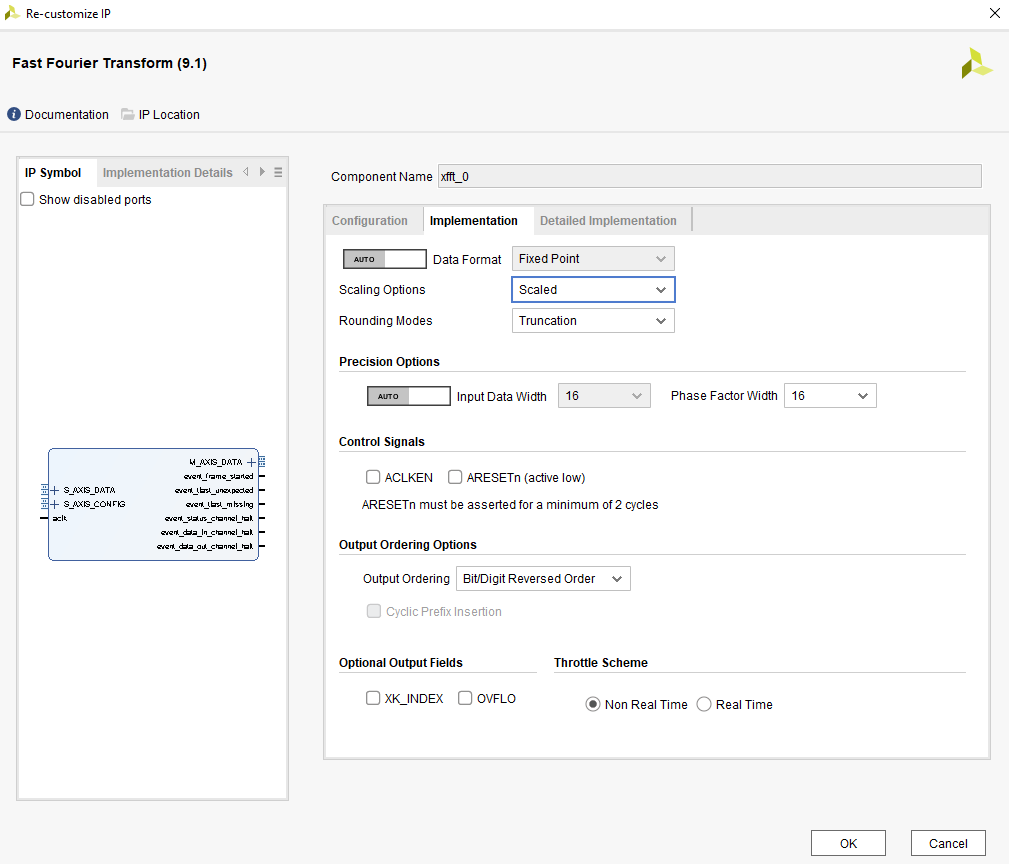
\includegraphics[width=0.5\textwidth]{image/fft_implemetation.png}
	\caption{Временная диаграмма работы интерфейса AXI4-Stream}
	\label{fft_implemetation}
\end{figure}
	
\section{Практическая часть}

\begin{figure}[h]
	\centering
	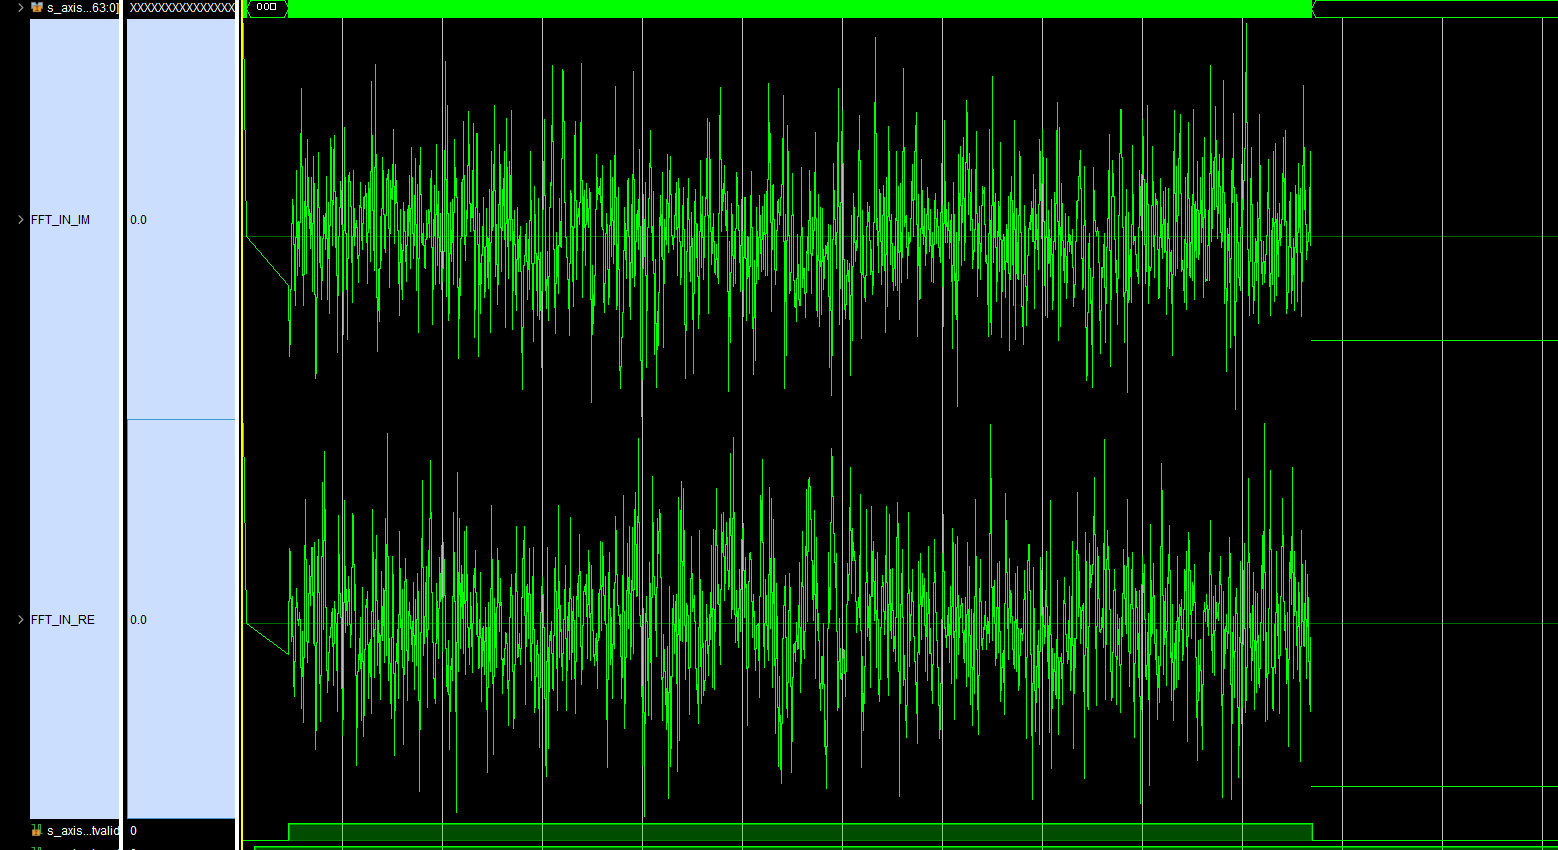
\includegraphics[width=0.5\textwidth]{image/lfm_with_noise.png}
	\caption{Временная диаграмма работы интерфейса AXI4-Stream}
	\label{fft_result}
\end{figure}
	
\begin{figure}[h]
	\centering
	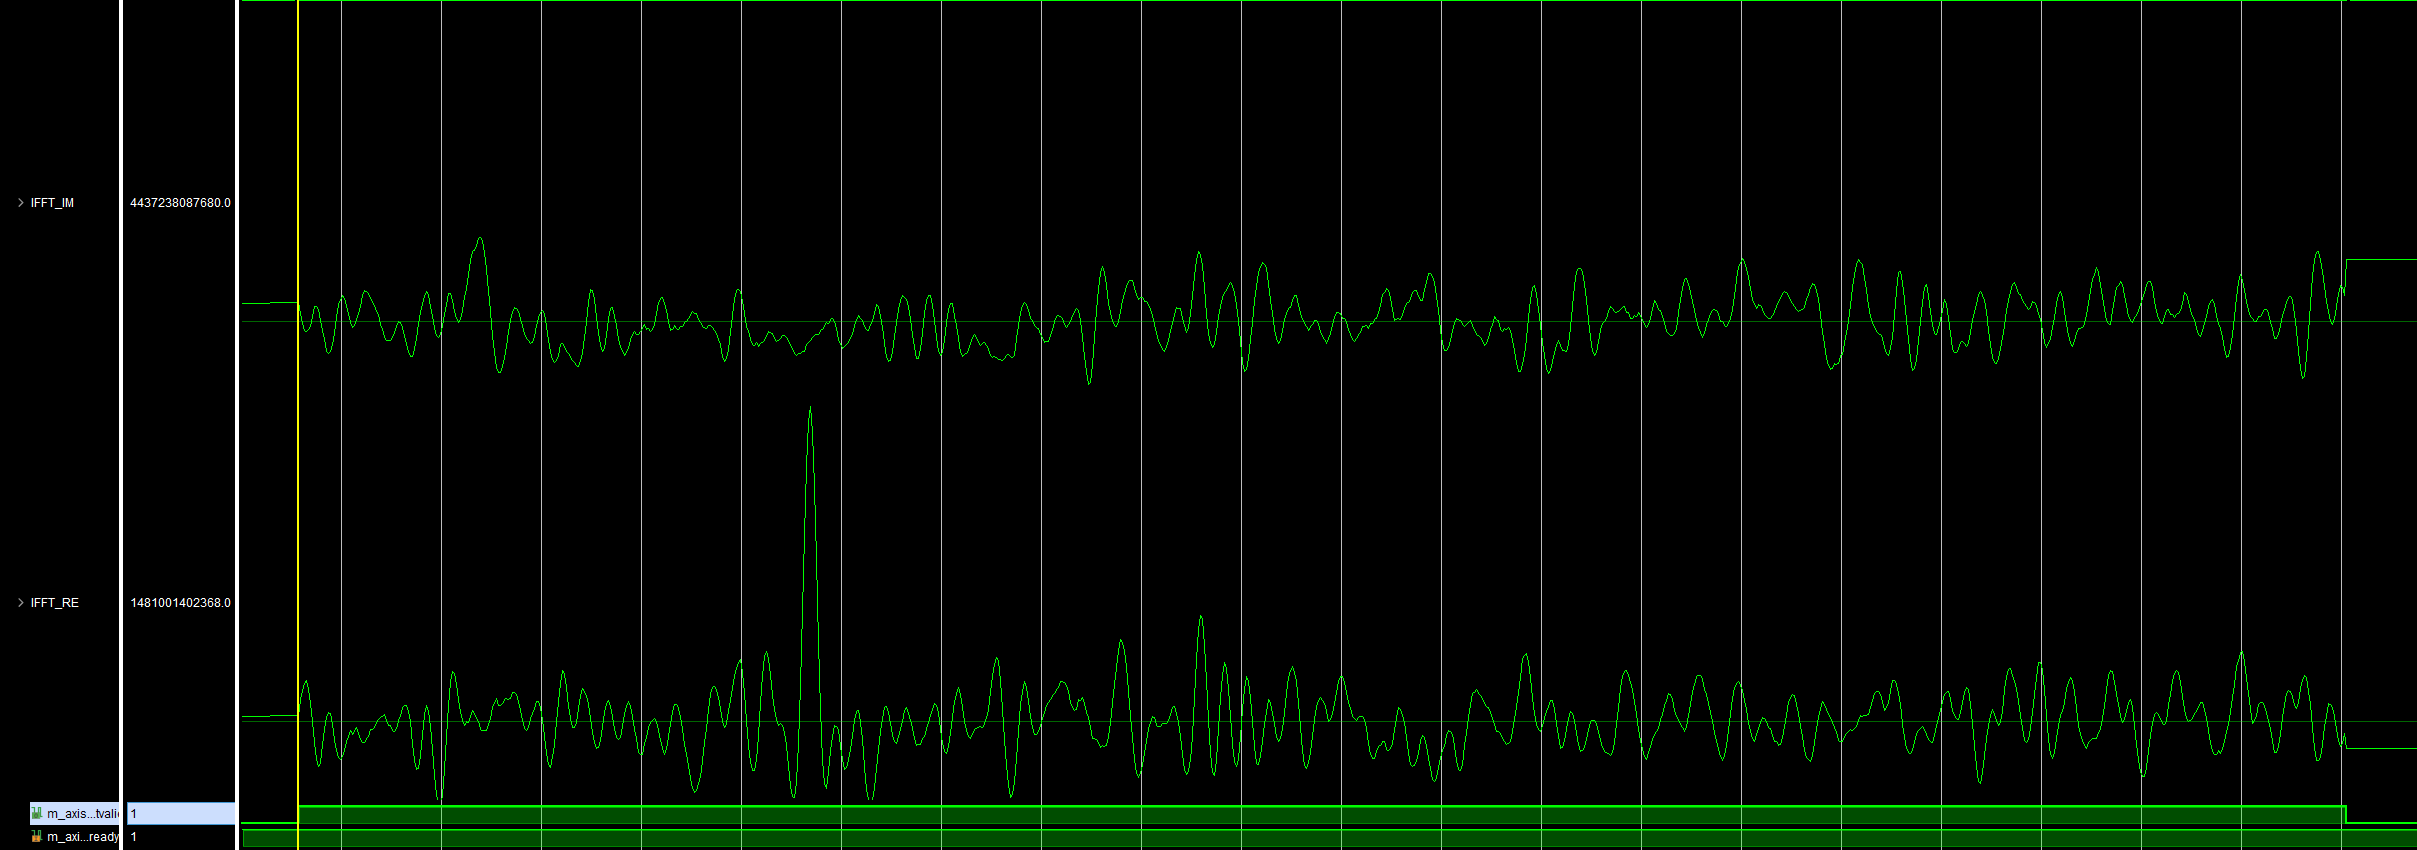
\includegraphics[width=0.5\textwidth]{image/correl_with_noise.png}
	\caption{Временная диаграмма работы интерфейса AXI4-Stream}
	\label{fft_detailed_implem}
\end{figure}